
%%%%%%%%%%%%%%%%%%%%%%%%%%%%%%%%%%%%%%%%%%%%%%%%%%%%%%%%%%%%
%%  This Beamer template was created by Cameron Bracken.
%%  Anyone can freely use or modify it for any purpose
%%  without attribution.
%%
%%  Last Modified: January 9, 2009
%%

\documentclass[xcolor={x11names,table},compress,svgnames,mathserif]{beamer}

%% General document %%%%%%%%%%%%%%%%%%%%%%%%%%%%%%%%%%
\usepackage{graphicx}
\usepackage{tikz}
\usepackage{spot}
\usetikzlibrary{mindmap}
\usetikzlibrary{decorations.fractals}
%\usepackage{lmodern}
\usepackage{animate}
\usepackage{movie15}
\usepackage{bm}
\usepackage{pifont}
\usepackage{smartdiagram}
\usepackage[customcolors]{hf-tikz}
\usepackage{empheq}
\usepackage[many]{tcolorbox}
\definecolor{pigment}{rgb}{0.2, 0.2, 0.6}
\definecolor{armygreen}{rgb}{0.29, 0.33, 0.13}
\usepackage{smartdiagram}
\usepackage{booktabs} % for table bottomrule and toprule
\usepackage{changepage} % shift tikzpicture horizontally

% highlight part of equation
\newcommand{\highlight}[1]{%
  \colorbox{red!50}{$\displaystyle#1$}}
  
  \newcommand{\highlights}[1]{%
  \colorbox{yellow!50}{$\displaystyle#1$}}


% for boxed equations
\usepackage{framed,color}
\definecolor{shadecolor}{rgb}{0.0,1.0,1.0}

\usepackage[absolute,overlay]{textpos}
\DeclareMathOperator*{\argmin}{arg\,min}

% boxed equaton
\usepackage[many]{tcolorbox}

\pgfdeclarehorizontalshading{section shading}{2cm}{
color(0cm)=(LightSlateGrey);
color(2cm)=(gray!7);
color(3cm)=(LightSlateGrey!15)
}

% Custom block environment
% Custom block environment
\newenvironment<>{varblock}[2][.9\textwidth]{%
  \setlength{\textwidth}{#1}
  \begin{actionenv}#3%
    \def\insertblocktitle{#2}%
    \par%
    \usebeamertemplate{block begin}}
  {\par%
    \usebeamertemplate{block end}%
  \end{actionenv}}
  
  %% Algorithm %%%%%
\usepackage[linesnumbered]{algorithm2e}
\newcommand{\nosemic}{\renewcommand{\@endalgocfline}{\relax}}% Drop semi-colon ;
\newcommand{\dosemic}{\renewcommand{\@endalgocfline}{\algocf@endline}}% Reinstate semi-colon ;
\newcommand{\pushline}{\Indp}% Indent
\newcommand{\popline}{\Indm\dosemic}% Undent
\newcommand{\shine}[1]{{\color{pigment}{#1}}} % use pigment color
\let\oldnl\nl% Store \nl in \oldnl
\newcommand{\nonl}{\renewcommand{\nl}{\let\nl\oldnl}}% Remove line number for one
\SetKwRepeat{Do}{do}{while}
%%%%%%%%%%%%%%%%%

% Vertical line between columns
\newcommand{\vdashrule}[1]{\tikz[remember picture]\draw[dashed,thick,overlay](current page.north)--+(0,-#1);}


%%%%%%%%%%%%%%%%%%%%%%%%%%%%%%%%%%%%%%%%%%%%%%%%%%%%%%

\usetikzlibrary{shapes,arrows,arrows.meta}
\usetikzlibrary{positioning,decorations.pathreplacing}
\tikzstyle{arrow} = [->,>=stealth, line width=1.2pt]
% Define block styles
\tikzstyle{decision} = [diamond, draw, fill=purple!20, 
    text width=5.0em, text badly centered, node distance=3cm, inner sep=0pt]
\tikzstyle{block} = [rectangle, draw=none, fill=blue!20, anchor=north, 
    text width=9.0em, text centered]
    \tikzstyle{blockr} = [rectangle, draw, fill=blue!20, 
    text width=9.0em, text centered, rounded corners]
\tikzstyle{line} = [draw, -latex']
\tikzstyle{cloud} = [draw=none, ellipse,fill=purple!20, node distance=3cm,
    minimum height=2em]
\tikzstyle{startstop} = [rectangle, draw, fill=DeepSkyBlue4,text=white,
   text width=4.5em, text centered, rounded corners]
 \tikzstyle{process} = [rectangle, draw, fill=DeepSkyBlue4,text=white,
   text width=9.0em, text centered]  
 \tikzstyle{io} = [trapezium, fill=DeepSkyBlue4,text=white, trapezium left angle=70, trapezium right angle=110, minimum width=2cm, text width=9.5em,minimum height=1cm, text centered, draw, inner sep=0pt]
    

%% Beamer Layout %%%%%%%%%%%%%%%%%%%%%%%%%%%%%%%%%%
\useoutertheme[subsection=false,shadow]{miniframes}
\useinnertheme{default}
%\usefonttheme{serif}
\usepackage{palatino}
\usepackage{xcolor}
\usepackage{amsmath,amsfonts,amssymb}

% Comparison chart on Slide 2
\usepackage{array,tabularx}
%\usepackage[most]{tcolorbox}

\setbeamerfont{title like}{shape=\scshape}
\setbeamerfont{frametitle}{shape=\scshape}
\setbeamertemplate{itemize items}[triangle] % if you wnat a circle
\setbeamertemplate{itemize subitem}[triangle]
\setbeamertemplate{navigation symbols}{}
%\setbeamertemplate{footline}[frame number]

\setbeamercolor{footlinecolor}{fg=white,bg=DeepSkyBlue4}
\defbeamertemplate*{footline}{infolines theme}
{
  \leavevmode%
  \hbox{%
  \begin{beamercolorbox}[wd=.333333\paperwidth,ht=2.25ex,dp=1ex,center]{footlinecolor}
 % {author in head/foot}%
    \usebeamerfont{author in head/foot}\insertshortauthor
   % \usebeamerfont{author in head/foot}\insertshortauthor~~(\insertshortinstitute)
  \end{beamercolorbox}%
  \begin{beamercolorbox}[wd=.333333\paperwidth,ht=2.25ex,dp=1ex,center]{title in head/foot}%
    \usebeamerfont{title in head/foot}\insertshorttitle
  \end{beamercolorbox}%
  \begin{beamercolorbox}[wd=.333333\paperwidth,ht=2.25ex,dp=1ex,right]{footlinecolor}
  %{date in head/foot}%
   % \usebeamerfont{date in head/foot}\insertshortdate{}\hspace*{2em}
    \usebeamerfont{date in head/foot}{manav.vohra@vanderbilt.edu}\hspace*{2em}
    \insertframenumber{} / \inserttotalframenumber\hspace*{2ex} 
  \end{beamercolorbox}}%
  \vskip0pt%
}
%\setbeamercolor{section in head/foot}{fg=white, bg=DeepSkyBlue4}

\setbeamercolor*{lower separation line head}{bg=DeepSkyBlue4} 
\setbeamercolor*{normal text}{fg=black,bg=white} 
\setbeamercolor*{alerted text}{fg=red} 
\setbeamercolor*{example text}{fg=black} 
\setbeamercolor*{structure}{fg=black} 
 
\setbeamercolor*{palette tertiary}{fg=black,bg=black!10} 
\setbeamercolor*{palette quaternary}{fg=black,bg=black!10} 

\renewcommand{\(}{\begin{columns}}
\renewcommand*\footnoterule{}
\renewcommand{\)}{\end{columns}}
\newcommand{\<}[1]{\begin{column}{#1}}
\renewcommand{\>}{\end{column}}

\newcommand*\subitem{%
  \item[\color{DeepSkyBlue4}\scalebox{0.6}{\ding{228}}]}
  
  \newcommand*\subitemtwo{%
  \item[\color{LightSlateGrey!15}\scalebox{0.6}{\ding{228}}]}

\newcommand*\myitem{%
  \item[\color{DeepSkyBlue4}\scalebox{0.6}{\ding{110}}]}
 
  \newcommand*\myitemtwo{%
  \item[\color{LightSlateGrey!15}\scalebox{0.6}{\ding{110}}]}
  
\newcommand*\Myitem{%
  \item[\color{DeepSkyBlue4}\scalebox{0.9}{\ding{42}}]}
  
\newcommand{\be}{\begin{equation}}
\newcommand{\ee}{\end{equation}}
\newcommand{\bea}{\begin{eqnarray}}
\newcommand{\eea}{\end{eqnarray}}
\newcommand{\p}{\partial}
\def\ol{\overline}
\def\no{\noindent}
\def\Vb{{\cal V}}
\def\Qd{\dot{Q}}
\newcommand{\angstrom}{\textup{\AA}}
%\DeclareMathSymbol{\ast}{\mathbin}{symbols}{"03}
 \newcommand{\argmax}{\operatornamewithlimits{arg\,max}}
 
 \setlength{\leftmargini}{0pt}
 

%---------------------QUOTATION--------------------------
\usepackage{etoolbox}
%\usepackage[svgnames]{xcolor}
\usepackage{framed}

% conditional for xetex or luatex
\newif\ifxetexorluatex
\ifxetex
  \xetexorluatextrue
\else
  \ifluatex
    \xetexorluatextrue
  \else
    \xetexorluatexfalse
  \fi
\fi
%
\ifxetexorluatex%
  \usepackage{fontspec}
  \usepackage{libertine} % or use \setmainfont to choose any font on your system
  \newfontfamily\quotefont[Ligatures=TeX]{Linux Libertine O} % selects Libertine as the quote font
\else
  \usepackage[utf8]{inputenc}
  \usepackage[T1]{fontenc}
  %\usepackage{libertine} % or any other font package
  \newcommand*\quotefont{\fontfamily{LinuxLibertineT-LF}} % selects Libertine as the quote font
\fi

\newcommand*\quotesize{30} % if quote size changes, need a way to make shifts relative
% Make commands for the quotes
\newcommand*{\openquote}
   {\tikz[remember picture,overlay,xshift=-3ex,yshift=-0.5ex]
   \node (OQ) {\quotefont\fontsize{\quotesize}{\quotesize}\selectfont``};\kern0pt}

\newcommand*{\closequote}[1]
  {\tikz[remember picture,overlay,xshift=-15ex,yshift={#1}]
   \node (CQ) {\quotefont\fontsize{\quotesize}{\quotesize}\selectfont''};}

% select a colour for the shading
\colorlet{shadecolor}{Azure}

\newcommand*\shadedauthorformat{\emph} % define format for the author argument

% Now a command to allow left, right and centre alignment of the author
\newcommand*\authoralign[1]{%
  \if#1l
    \def\authorfill{}\def\quotefill{\hfill}
  \else
    \if#1r
      \def\authorfill{\hfill}\def\quotefill{}
    \else
      \if#1c
        \gdef\authorfill{\hfill}\def\quotefill{\hfill}
      \else\typeout{Invalid option}
      \fi
    \fi
  \fi}
% wrap everything in its own environment which takes one argument (author) and one optional argument
% specifying the alignment [l, r or c]
%
\newenvironment{shadequote}[2][l]%
{\authoralign{#1}
\ifblank{#2}
   {\def\shadequoteauthor{}\def\yshift{-2ex}\def\quotefill{\hfill}}
   {\def\shadequoteauthor{\par\authorfill\shadedauthorformat{#2}}\def\yshift{2ex}}
\begin{snugshade}\begin{quote}\openquote}
{\shadequoteauthor\quotefill\closequote{\yshift}\end{quote}\end{snugshade}}


%%%%%%%%%%%%%%%%%%%%%%%%%%%%%%%%%%%%%%%%%%%%%%%%%%

\title[AM Defects: PCAS Method]{\textbf{A Fast Supervised Learning Method for
High-Dimensional Problems}}
\thispagestyle{empty}
\pgfsetfillopacity{0.9}
\setbeamercolor{title}{bg=DeepSkyBlue4,fg=white}


%\subtitle{SUBTITLE}
\author[M. Vohra]{\vspace{-3mm}Manav Vohra, Paromita Nath, Sankaran Mahadevan}

%\scriptsize
\institute{ 
%Vanderbilt University\\ \vspace{1mm}

\includegraphics[width=0.12\textwidth]{./Figures/VU}}

\date{\scriptsize\today}


\begin{document}


%___________________________NEW SLIDE______________________________________
{
\setbeamertemplate{headline}{}

\begin{frame}[noframenumbering]

\titlepage
\vspace{-21mm}
\centering

\end{frame}
}

%___________________________NEW SLIDE______________________________________

\begin{frame}{Principal Component--Active Subspace (PCAS) Method}

\begin{center}
\begin{figure}[htbp]
\begin{tikzpicture}[node distance=1.2cm,scale=0.6, every node/.style={scale=0.65}]

\node (field) [io, text width=6em] {Field Data\\ $\mathcal{S}\in\mathbb{R}^N$};

\node (pca) [process, right of=field, text width=14em, xshift=6.0cm] {Optimal $\#$ of features\\ $z_k$, $k=1,\ldots,K$\\
$\mathbb{R}^{N}\rightarrow \mathbb{R}^{K},~K\ll N$};

\draw [arrow] (field) -- node[anchor=south] {PCA} (pca);

\node (zk) [process, below of=pca, text width=13em, yshift=-3.0cm] {$z_k=f(\bm{\theta_p},\bm{\theta_m})$\\
$\bm{\theta_p}$: Process Parameters\\ $\bm{\theta_m}$: Material Properties\\
$\bm{\theta}$ = $\{\bm{\theta_p},\bm{\theta_m}\}\in\mathbb{R}^{N_m+N_p}$};

\draw [arrow] (pca) -- (zk);

\node (as) [io, below of=field, text width=7em, yshift=-3.0cm]{\vspace{0.5mm}$z_k(\bm{\theta})=G(\eta)$\\ $\eta=
\bm{\theta}^\top \bm{W_1}$\\ $\mathbb{R}^{N_m+N_p}\rightarrow \mathbb{R}^{N_\eta}$\\
$(N_m+N_p)\ll N_\eta$\vspace{0.5mm}};

\draw [arrow] (zk) -- node [above] {Subspace} node [below] {Computation} (as);

\draw [arrow,dashed] (as) -- (field);

\end{tikzpicture}
\end{figure}
\vspace{5mm}

$G(\eta)\rightarrow z_k(\bm{\theta})\rightarrow \mathcal{S}$

\end{center}

\end{frame}

%___________________________NEW SLIDE______________________________________

\begin{frame}{Finite Element Model}

\begin{columns}
\begin{column}{0.5\textwidth}

Heat Transfer:
\vspace{-2mm}
\be
\rho C_p(T) = \nabla\cdot \bm{q} (\bm{r},t) +Q(\bm{r},t) \nonumber
\ee
\vspace{-5mm}
\be
\bm{q} = -\kappa(T)\nabla T \nonumber
\ee
\vspace{-3mm}
\be
Q = f(z,P)\exp(f(x,y,v)) \nonumber
\ee
\begin{center}
\scriptsize{$P$: Laser Power~(W), $v$: Scan speed~(m/s)}
\end{center}

Stress Calculation:


\end{column}

\begin{column}{0.5\textwidth}
\begin{figure}[htbp]
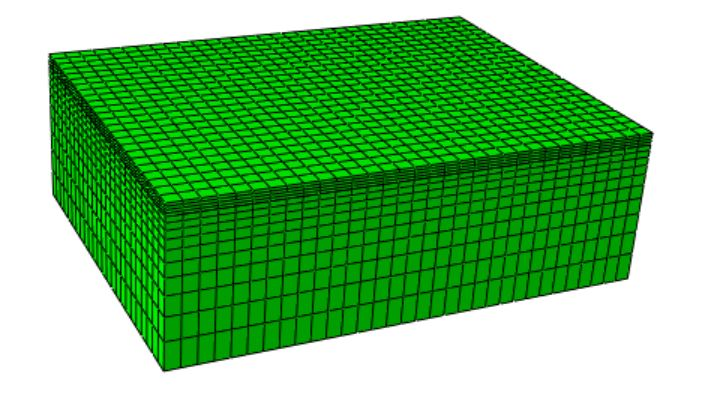
\includegraphics[width=0.85\textwidth]{./Figures/mesh}
\end{figure}
\vspace{2mm}
\begin{figure}[htbp]
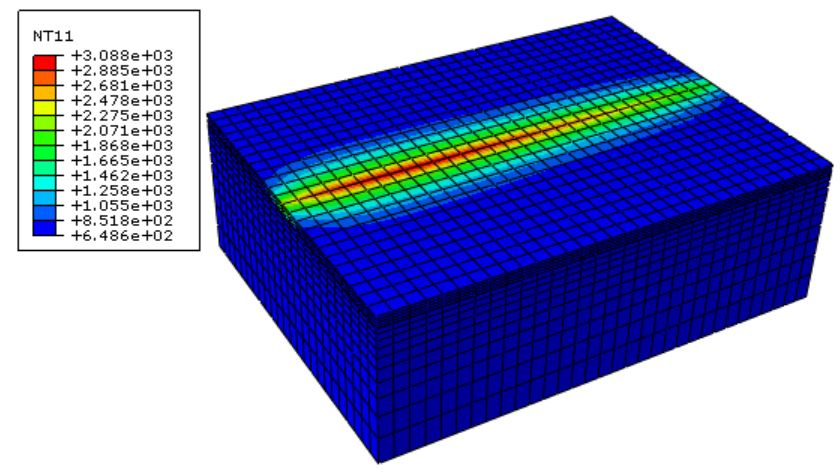
\includegraphics[width=0.85\textwidth]{./Figures/source}
\end{figure}
\end{column}
\end{columns}

\end{frame}

%___________________________NEW SLIDE______________________________________

\begin{frame}{Residual Stress Field}

\begin{columns}
\begin{column}{0.5\textwidth}

Principal Component Analysis

\begin{figure}[htbp]
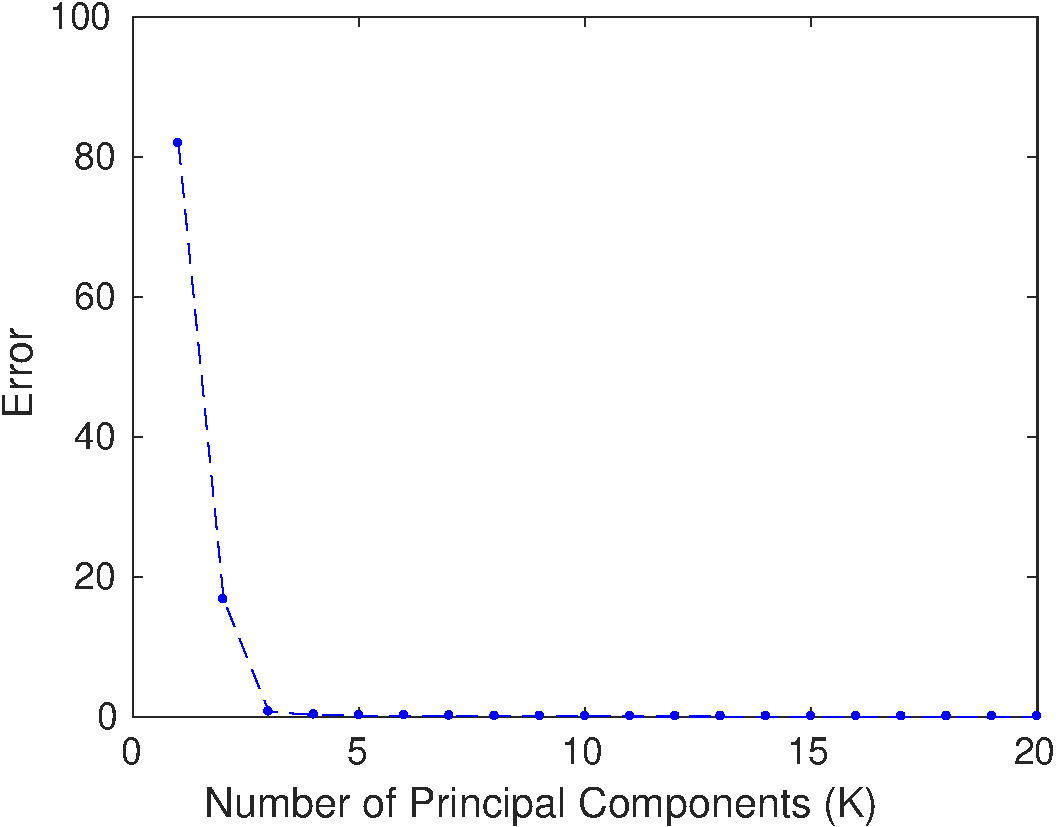
\includegraphics[width=0.65\textwidth]{./Figures/error_k}
\end{figure}

\rowcolors{2}{black!20}{white}
\resizebox{6cm}{!}{
  \begin{tabular}{ll}
 % \scriptsize
    \rowcolor{black}
    {\color{white}\scriptsize{Parameter}} & {\color{white} \scriptsize{Nominal Value}} \\
    \scriptsize{Scan Speed, $v$ (mm/s)} & \scriptsize{500} \\
   \scriptsize{Laser Power, $P$ (W)} & \scriptsize{160} \\
    \scriptsize{Pre-heat Temperature, $T_0$ (C)} & \scriptsize{650} \\
     \scriptsize{Yield Strength, $Y$ (MPa)} & \scriptsize{825} \\
      \scriptsize{Elastic Strength, $E$ (GPa)} & \scriptsize{110} \\
       \scriptsize{Density, $\rho$ (kg/m$^3$)} & \scriptsize{4428} \\
        \scriptsize{Specific heat, $C_p = C_0 + C_1T+C_2T^2$ (J/kg/K)} & \scriptsize{540, 0.43, -3.2$\times 10^{-5}$}\\
        \scriptsize{Thermal Conductivity, $\kappa = D_0 + D_1T+D_2T^2$ (W/m/K)} & \scriptsize{7.2, 0.011, 1.4$\times 10^{-6}$}
     \end{tabular}
     }

\end{column}

\begin{column}{0.5\textwidth}
\begin{figure}[htbp]
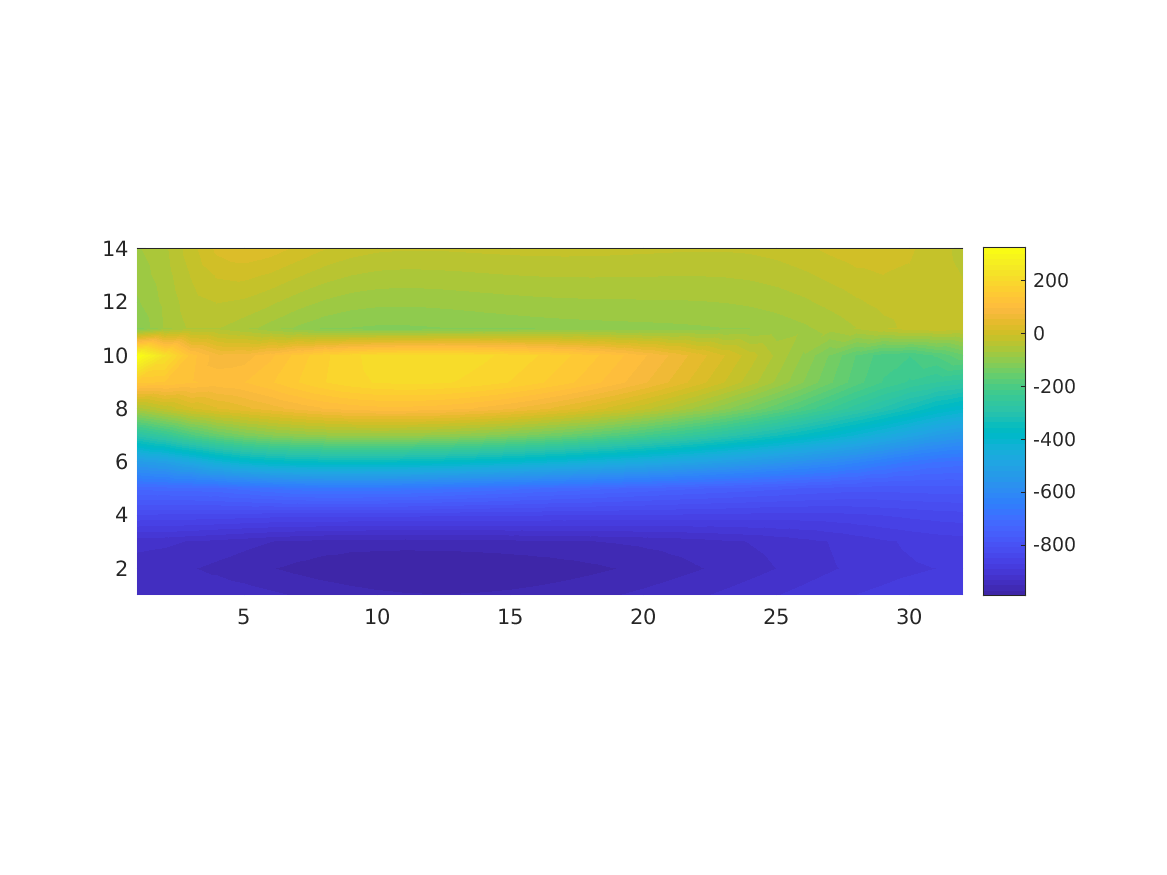
\includegraphics[width=0.95\textwidth]{./Figures/origZ_sam20}
\end{figure}
\vspace{-15mm}
\begin{figure}[htbp]
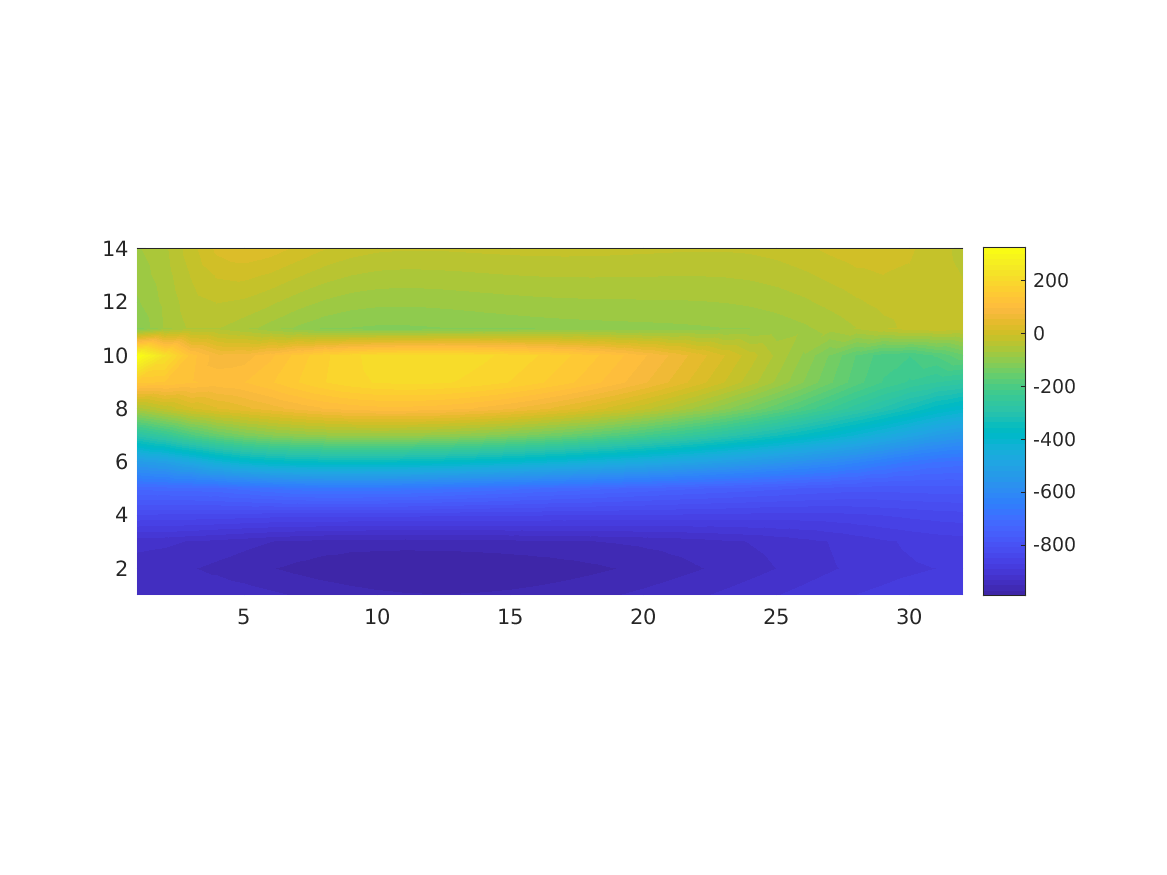
\includegraphics[width=0.95\textwidth]{./Figures/recZ_sam20}
\\ \vspace{-10mm} \scriptsize{$\mathbb{R}^{32\times 14}\rightarrow\mathbb{R}^3(K=3)$}
\end{figure}
\end{column}
\end{columns}

\end{frame}

%___________________________NEW SLIDE______________________________________

\begin{frame}{Active Subspace Discovery}

\begin{columns}
\begin{column}{0.33\textwidth}
\begin{figure}[htbp]
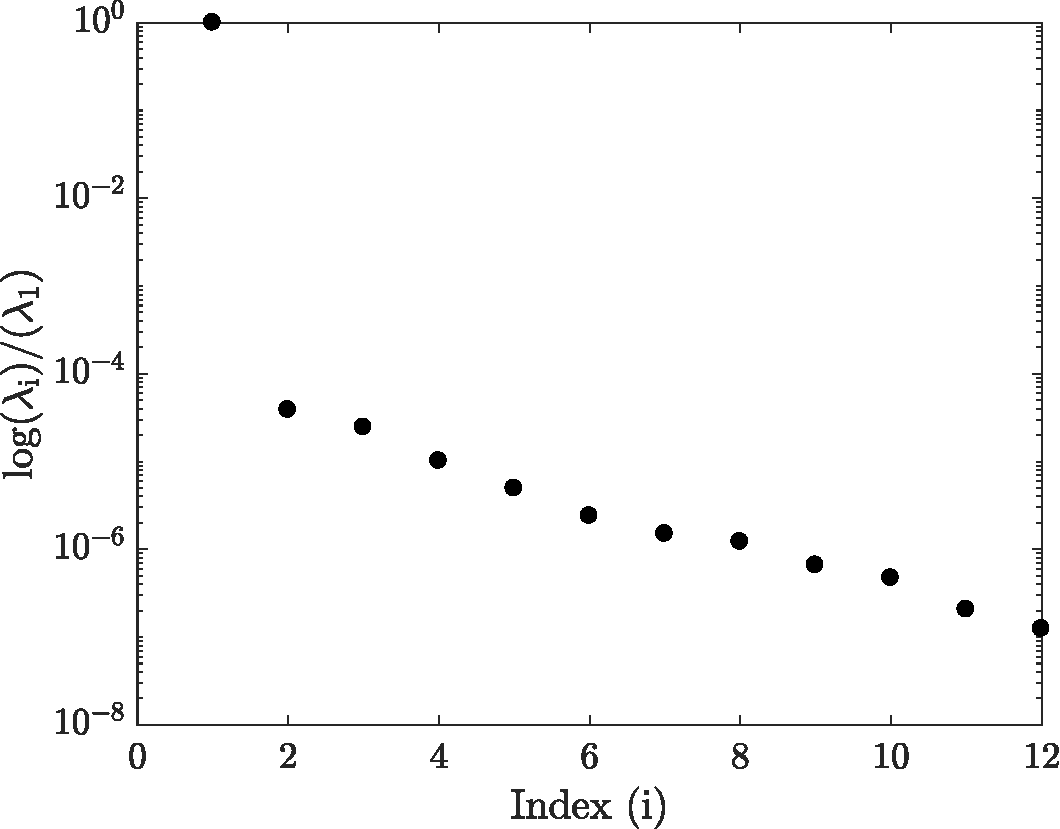
\includegraphics[width=0.95\textwidth]{./Figures/eig_Zf1}\\
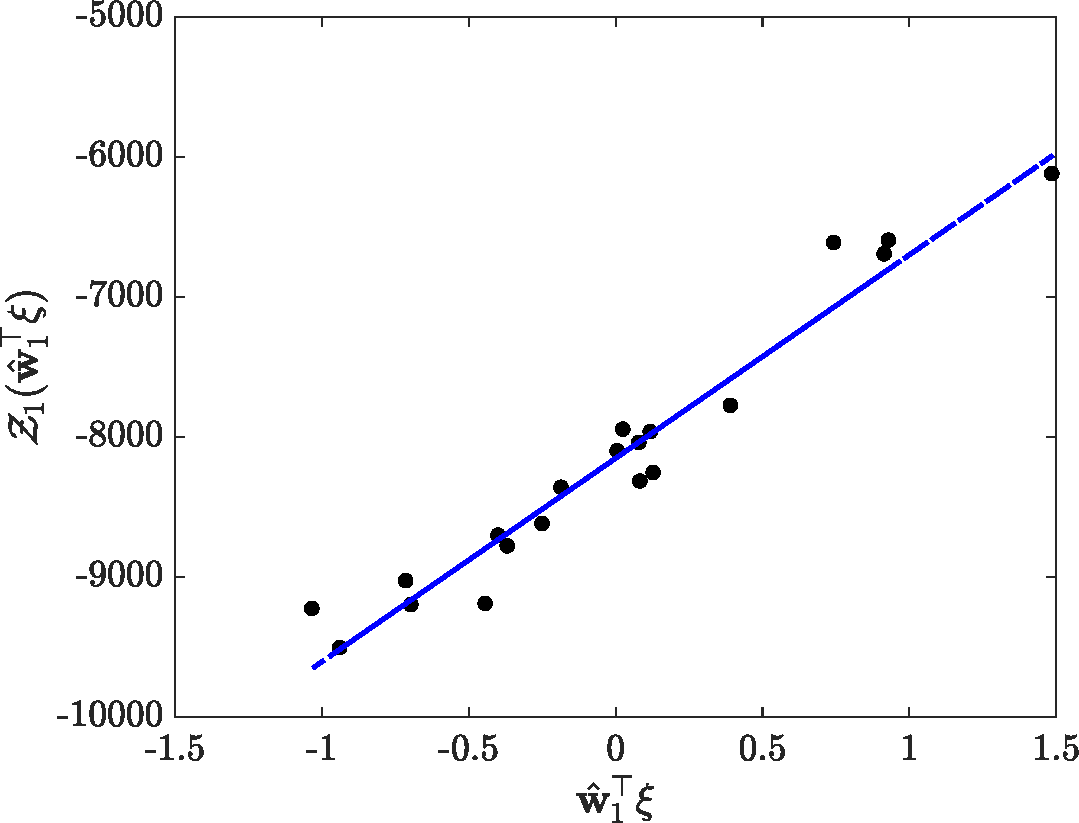
\includegraphics[width=0.95\textwidth]{./Figures/SSP_Zf1}
\end{figure}
\end{column}

\begin{column}{0.33\textwidth}
\begin{figure}[htbp]
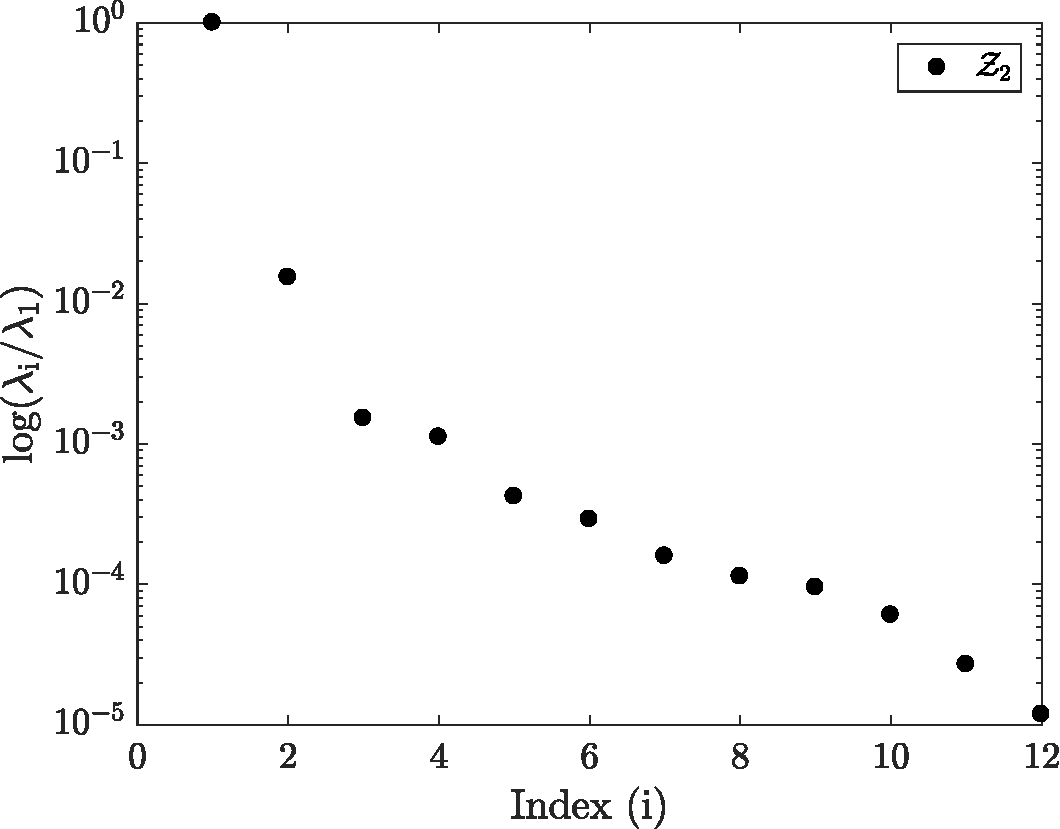
\includegraphics[width=0.95\textwidth]{./Figures/eig_Zf2}\\
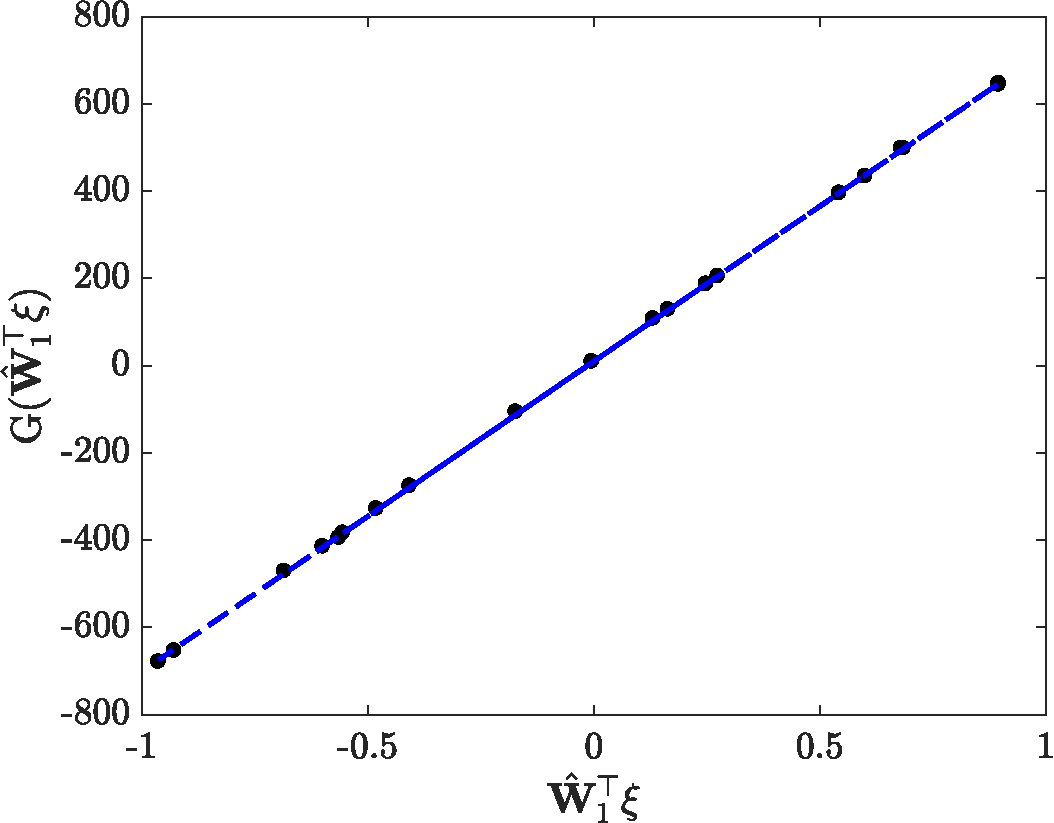
\includegraphics[width=0.95\textwidth]{./Figures/SSP_Zf2}
\end{figure}
\end{column}

\begin{column}{0.33\textwidth}
\begin{figure}[htbp]
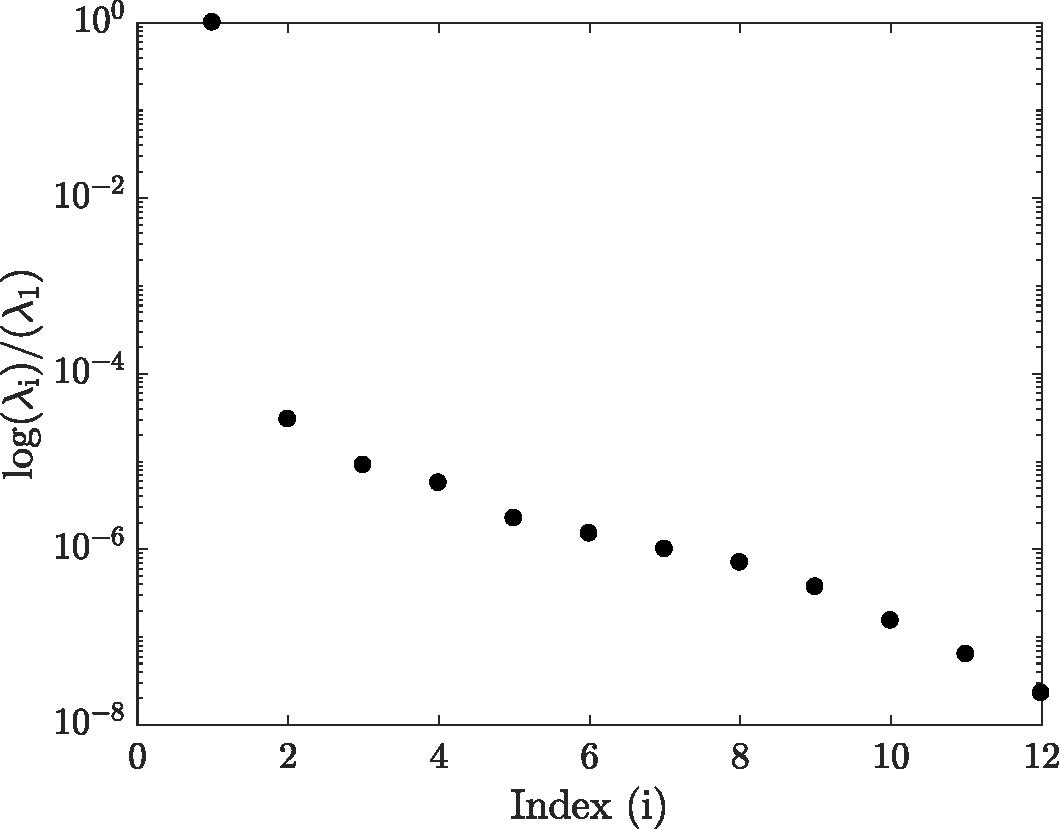
\includegraphics[width=0.95\textwidth]{./Figures/eig_Zf3}\\
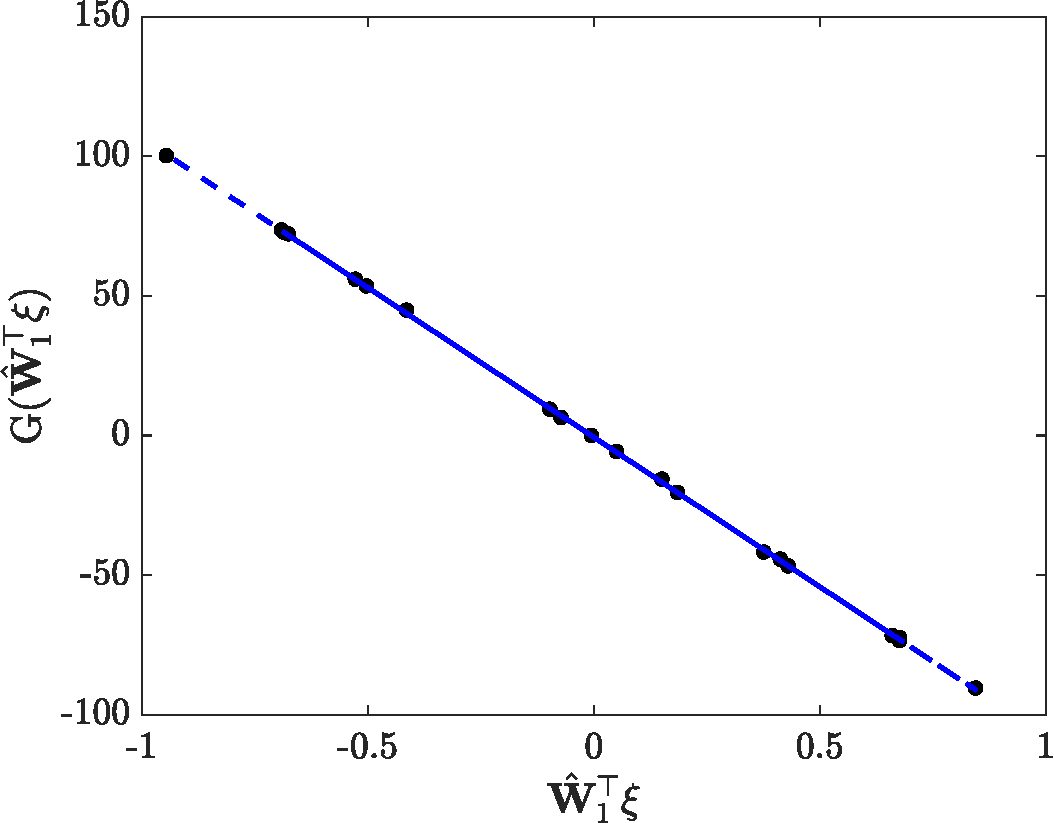
\includegraphics[width=0.95\textwidth]{./Figures/SSP_Zf3}
\end{figure}
\end{column}
\end{columns}

\end{frame}

%___________________________NEW SLIDE______________________________________

\begin{frame}{GSA: Activity Scores}

\begin{shaded}
%\vspace{-5mm}
\scriptsize
\centering
\be
\nu_{i,r}(f) = \sum\limits_{j=1}^{r} \lambda_j w_{i,j}^2, i=1,\ldots,N_p \nonumber
\ee
%\vspace{-7mm}
\end{shaded}

\begin{columns}
\begin{column}{0.33\textwidth}
\begin{figure}[htbp]
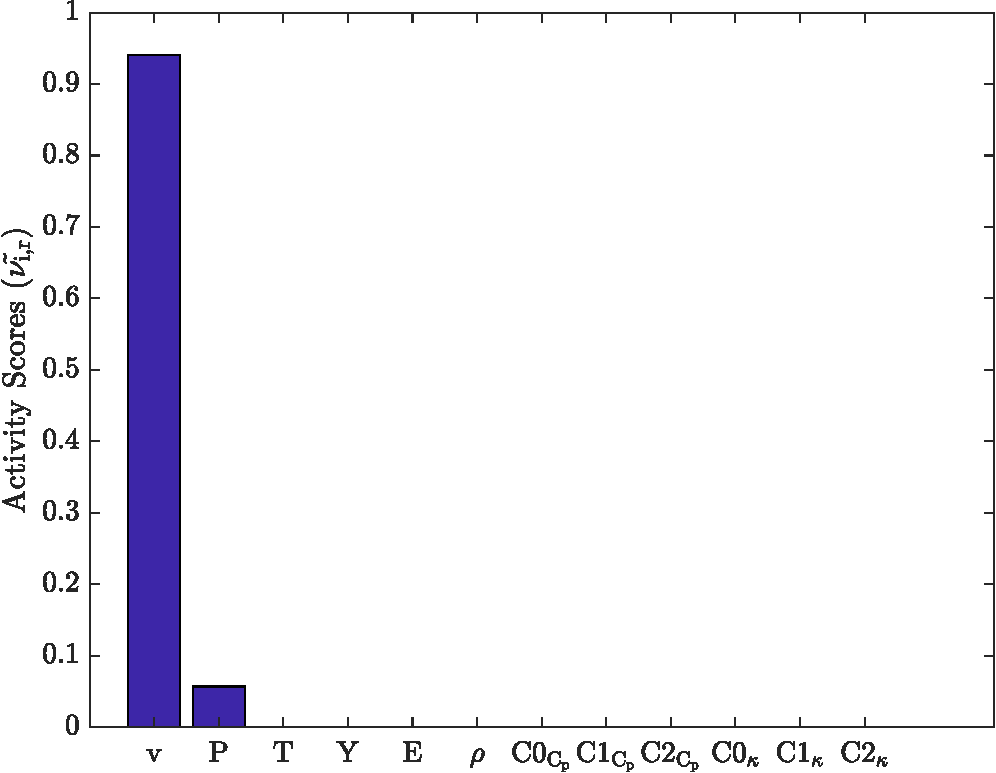
\includegraphics[width=0.95\textwidth]{./Figures/as_Zf1}\\
\end{figure}
\end{column}

\begin{column}{0.33\textwidth}
\begin{figure}[htbp]
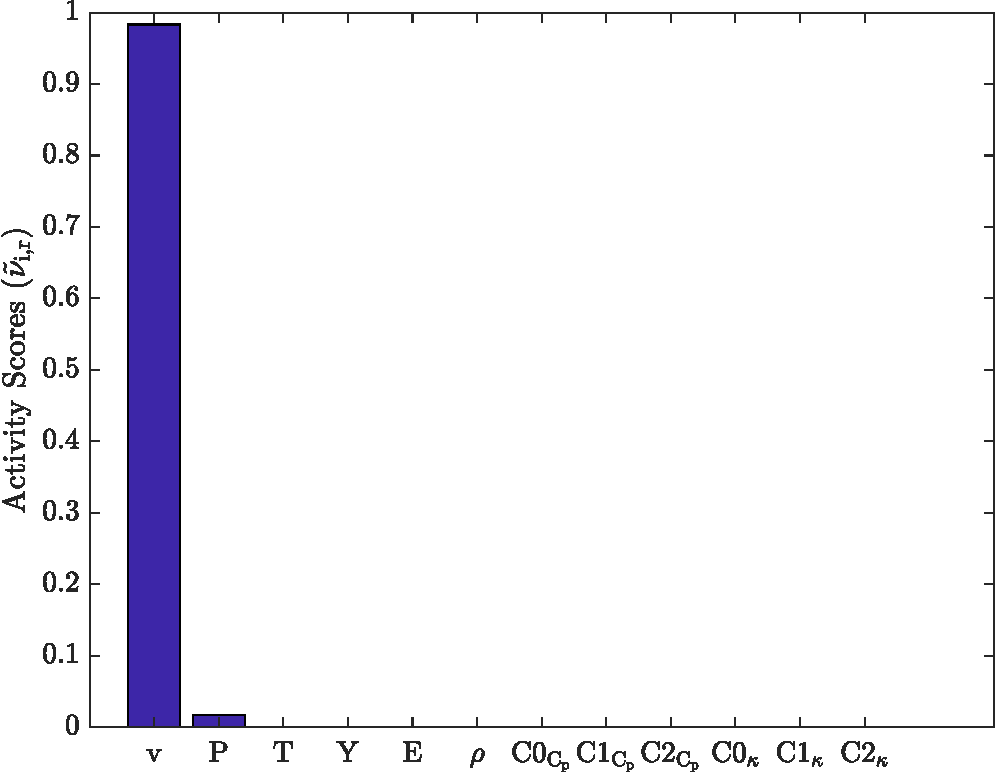
\includegraphics[width=0.95\textwidth]{./Figures/as_Zf2}\\
\end{figure}
\end{column}

\begin{column}{0.33\textwidth}
\begin{figure}[htbp]
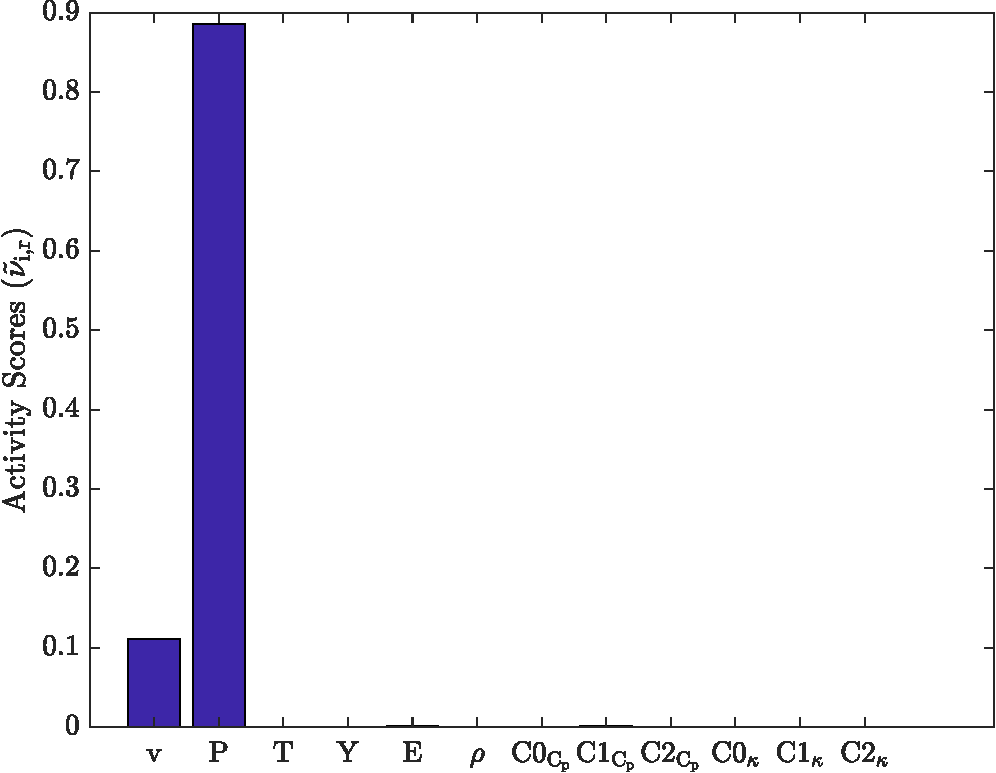
\includegraphics[width=0.95\textwidth]{./Figures/as_Zf3}\\
\end{figure}
\end{column}
\end{columns}

\end{frame}

\end{document}
